%\chapter{Название второй главы: разработка метода, алгоритма, модели исследования} \label{ch2}
	
% не рекомендуется использовать отдельную section <<введение>> после лета 2020 года
%\section{Введение} \label{ch2:intro}
\chapter{Разработка архитектуры модели и описание используемых методов} \label{ch2}

\noindent
В данной главе представлена разработанная архитектура модели глубокого 
обучения для прогнозирования фенотипических признаков по SNP-данным. 
Подробно описываются все компоненты предложенной модели: блок 
генетического кодирования, трансформерный блок, блок прогнозирования, 
а также реконструкционный блок, выполняющий функцию регуляризации. 
Для каждого блока приводится математическое описание преобразований 
и обоснование принятых архитектурных решений. Помимо архитектуры, 
в главе рассматриваются методы аугментации данных и настройки процесса 
обучения. В параграфе \ref{ch2:architecture} представлено детальное 
описание архитектуры модели и её ключевых компонентов.\cite{ctan-biblatex-gost}

\section{Архитектура модели}
\label{ch2:architecture}

Разработанная модель реализована с использованием библиотеки PyTorch 
и представляет собой последовательное соединение четырёх основных 
логических блоков, которые преобразуют исходные SNP-данные в предсказания 
фенотипических признаков. Общая схема архитектуры показана на рисунке 
\ref{fig:model_architecture}.

\begin{figure}
	\centering
	
\includegraphics[width=0.4\textwidth]{model_overview_highres.png}
	\caption{Общая архитектура предложенной модели}
	\label{fig:model_architecture}
\end{figure}

\subsection{Блок генетического кодирования (GeneticEncodingBlock)}

Блок генетического кодирования выполняет преобразование входных SNP-данных 
в векторные представления на уровне генов. Основная задача этого блока 
состоит в агрегировании информации о SNP, относящихся к одному гену, 
с учётом их значений, позиционной информации и обучаемых весов.

\paragraph{Сопоставление SNP с генами}

На первом этапе блок использует таблицу соответствия SNP генам, которая 
формируется на основе аннотации генома. Для каждого SNP определяется ген, 
к которому он относится (т.е. в пределах которого или в регуляторной 
области которого данный SNP локализован), после чего строится структура 
данных, позволяющая группировать SNP по соответствующим генам. Пусть 
$G$~--- множество всех генов, $|G| = N_{\text{genes}}$. Для каждого гена 
$g \in G$ определено множество индексов SNP $S_g = \{i : \text{SNP}_i 
\text{ относится к гену } g\}$.

\paragraph{Частотное кодирование SNP}

Перед агрегацией значения SNP подвергаются частотному кодированию. Исходные 
значения $\{0,1,2\}$ заменяются частотами встречаемости соответствующих 
аллелей в обучающей выборке:
\[
\tilde{x}_{ij} = \frac{\text{count}(x_{ij})}{n},
\]
где $\text{count}(x_{ij})$~--- количество образцов со значением $x_{ij}$ 
для $j$-го SNP. Такое кодирование позволяет привести данные к единому 
масштабу и учесть редкость некоторых аллелей.

\paragraph{Механизм внимания на уровне SNP}

Ключевой особенностью разработанной модели является использование 
механизма внимания для адаптивной агрегации SNP внутри каждого гена. 
В отличие от простого усреднения или свёртки, механизм внимания позволяет 
модели выделять наиболее информативные SNP-маркеры и подавлять шумовые 
компоненты.

Для каждого гена $g$ и относящегося к нему SNP $s \in S_g$ формируется 
векторное представление:
\[
\mathbf{h}_{gs} = \tilde{x}_{gs} \cdot \mathbf{w}_{\text{snp}}, \quad
\mathbf{w}_{\text{snp}} \in \mathbb{R}^d,
\]
где $d$~--- размерность эмбеддинга, $\mathbf{w}_{\text{snp}}$~--- обучаемый 
вектор, общий для всех SNP. Далее для каждого SNP вычисляется скалярная 
оценка важности:
\[
e_{gs} = \mathbf{a}^{\top} \mathbf{h}_{gs}, \quad \mathbf{a} \in \mathbb{R}^d,
\]
где $\mathbf{a}$~--- обучаемый вектор параметров внимания. Нормированные 
коэффициенты внимания получаются применением функции softmax:
\[
\alpha_{gs} = \frac{\exp(e_{gs})}{\sum_{k \in S_g} \exp(e_{gk})}.
\]

Адаптивное представление гена формируется как взвешенная сумма векторных 
представлений SNP:
\[
\mathbf{v}_g = \sum_{s \in S_g} \alpha_{gs} \mathbf{h}_{gs}.
\]

Такой подход позволяет модели самостоятельно определять, какие SNP вносят 
наибольший вклад в формирование фенотипического признака, и усиливать их 
сигнал.

\paragraph{Обучаемые эмбеддинги генов}

Каждый ген имеет собственный обучаемый эмбеддинг $\mathbf{e}_g \in \mathbb{R}^d$, 
который позволяет модели учитывать индивидуальные особенности гена, 
не зависящие от конкретных SNP-значений в образце.

\paragraph{Позиционное кодирование}

Для учёта физического расположения генов на хромосомах используется 
позиционное кодирование. В отличие от стандартного подхода, в данной 
работе позиция гена масштабируется с учётом его средней SNP-активности:
\[
p_g^{\text{scaled}} = \rho \cdot \text{pos}_g \cdot \exp(\bar{x}_g),
\]
где $\text{pos}_g$~--- репрезентативная позиция гена на хромосоме, 
вычисляемая как среднее арифметическое координат начала и конца 
кодирующей области: $\text{pos}_g = (\text{start}_g + \text{end}_g) / 2$; 
$\bar{x}_g = \frac{1}{|S_g|} \sum_{s \in S_g} \tilde{x}_{gs}$~--- среднее 
значение SNP в гене, $\rho$~--- масштабирующий коэффициент.

Позиционное кодирование для $g$-го гена и $j$-й координаты эмбеддинга 
вычисляется по формулам:
\[
\text{PE}_{g,2k} = \sin\left(p_g^{\text{scaled}} \cdot 
\exp\left(-\frac{\ln 10^5}{d} \cdot k\right)\right),
\]
\[
\text{PE}_{g,2k+1} = \cos\left(p_g^{\text{scaled}} \cdot 
\exp\left(-\frac{\ln 10^5}{d} \cdot k\right)\right),
\]
где $k = 0, 1, \dots, d/2 - 1$. Такое кодирование позволяет модели 
различать гены по их хромосомному положению, при этом гены с более 
высокой вариативностью SNP получают усиленный позиционный сигнал.

\paragraph{Итоговое представление гена}

Финальное представление гена формируется как сумма трёх компонентов:
\[
\mathbf{z}_g = \mathbf{v}_g + \mathbf{e}_g + \mathbf{PE}_g,
\]
где $\mathbf{v}_g$~--- агрегированное SNP-представление, $\mathbf{e}_g$~--- 
обучаемый эмбеддинг гена, $\mathbf{PE}_g$~--- позиционное кодирование.

Для стабилизации обучения после суммирования применяется Layer Normalization:
\[
\mathbf{z}_g^{\text{norm}} = \text{LayerNorm}(\mathbf{z}_g).
\]

Выходом блока генетического кодирования является тензор размерности 
$[B, N_{\text{genes}}, d]$, где $B$~--- размер батча (количество образцов 
растений в одной итерации обучения), $N_{\text{genes}}$~--- количество 
генов, $d$~--- размерность эмбеддинга. Таким образом, для каждого образца 
формируется матрица признаков размера $N_{\text{genes}} \times d$, которая 
затем поступает на вход трансформерному блоку.

\subsection{Трансформерный блок (TransformerBlock)}

Трансформерный блок предназначен для моделирования сложных межгенных 
взаимодействий. Он обрабатывает последовательность векторных представлений 
генов и выявляет зависимости между удалёнными генетическими регионами.

\paragraph{Механизм многоголового самовнимания}

В основе трансформерного блока лежит механизм многоголового самовнимания.\cite{Vaswani2017} Для входной последовательности $\mathbf{Z} \in \mathbb{R}^{B \times N_{\text{genes}} \times d}$ 
вычисляются три матрицы: запросов $\mathbf{Q}$, ключей $\mathbf{K}$ и 
значений $\mathbf{V}$:
\[
\mathbf{Q} = \mathbf{Z} \mathbf{W}^Q, \quad
\mathbf{K} = \mathbf{Z} \mathbf{W}^K, \quad
\mathbf{V} = \mathbf{Z} \mathbf{W}^V,
\]
где $\mathbf{W}^Q, \mathbf{W}^K, \mathbf{W}^V \in \mathbb{R}^{d \times d}$~--- 
обучаемые матрицы проекций.

Внимание для одной головы вычисляется как:
\[
\text{Attention}(\mathbf{Q}, \mathbf{K}, \mathbf{V}) = 
\text{softmax}\left(\frac{\mathbf{Q} \mathbf{K}^\top}{\sqrt{d_k}}\right) \mathbf{V},
\]
где $d_k = d/h$~--- размерность головы, $h$~--- количество голов внимания.

Механизм многоголовости позволяет модели анализировать взаимосвязи между 
генами с разных ракурсов:
\[
\text{MultiHead}(\mathbf{Z}) = \text{Concat}(\text{head}_1, \dots, \text{head}_h) \mathbf{W}^O,
\]
где каждая голова работает со своей проекцией входных данных, а 
$\mathbf{W}^O \in \mathbb{R}^{d \times d}$~--- обучаемая матрица проекции 
объединённого результата.

\paragraph{Механизм dropout}

Для предотвращения переобучения в каждом слое трансформера используется 
механизм dropout \cite{Srivastava2014}. Dropout случайным образом 
обнуляет долю нейронов (с вероятностью $p_{\text{dropout}} = 0.2$) на 
каждой итерации обучения, что вынуждает сеть не полагаться на отдельные 
нейроны и способствует формированию более робастных представлений.

\paragraph{Полносвязная сеть}

После слоя внимания результат проходит через двухслойную полносвязную сеть 
с функцией активации GELU:
\[
\text{FFN}(\mathbf{X}) = \text{GELU}(\mathbf{X} \mathbf{W}_1 + \mathbf{b}_1) \mathbf{W}_2 + \mathbf{b}_2,
\]
где $\mathbf{W}_1 \in \mathbb{R}^{d \times d_{\text{ff}}}$, 
$\mathbf{W}_2 \in \mathbb{R}^{d_{\text{ff}} \times d}$, $d_{\text{ff}}$~--- 
размерность скрытого слоя feed-forward сети.

\paragraph{Остаточные соединения и нормализация}

Для улучшения сходимости и предотвращения затухания градиентов используются 
остаточные соединения и Layer Normalization. Каждый подблок трансформера 
имеет структуру:
\[
\mathbf{Z}' = \text{LayerNorm}(\mathbf{Z} + \text{MultiHead}(\mathbf{Z})),
\]
\[
\mathbf{Z}'' = \text{LayerNorm}(\mathbf{Z}' + \text{FFN}(\mathbf{Z}')).
\]

Выходом трансформерного блока является тензор той же размерности 
$[B, N_{\text{genes}}, d]$, содержащий контекстуализированные представления 
генов с учётом их взаимосвязей.

\subsection{Блок прогнозирования (PredictionBlock)}

Блок прогнозирования преобразует выход трансформера в предсказания 
фенотипических признаков. В отличие от базовой архитектуры, где применялось 
прямое разворачивание всех генов в вектор, в данной работе используется 
гибридный механизм агрегации.

\paragraph{Гибридная агрегация с CLS-токеном}

В начало последовательности генов добавляется специальный CLS-токен, 
который агрегирует глобальную информацию о геноме. После обработки 
трансформером этот токен содержит контекстуализированное представление 
всего генома.

Пусть $\mathbf{z}_{\text{CLS}}$~--- представление CLS-токена, а 
$\{\mathbf{z}_g\}_{g=1}^{N_{\text{genes}}}$~--- представления генов после 
трансформерного блока. Вычисляются веса внимания для генов:
\[
a_g = \frac{\exp(\mathbf{u}^{\top} \mathbf{z}_g)}{\sum_{k=1}^{N_{\text{genes}}} 
	\exp(\mathbf{u}^{\top} \mathbf{z}_k)}, \quad \mathbf{u} \in \mathbb{R}^d,
\]
\[
\mathbf{z}_{\text{attn}} = \sum_{g=1}^{N_{\text{genes}}} a_g \mathbf{z}_g.
\]

Итоговое агрегированное представление формируется как взвешенная сумма 
представления CLS-токена и представления, полученного с помощью механизма 
внимания:
\[
\mathbf{z}_{\text{final}} = \alpha \cdot \mathbf{z}_{\text{CLS}} + 
(1 - \alpha) \cdot \mathbf{z}_{\text{attn}},
\]
где $\alpha \in [0,1]$~--- обучаемый параметр баланса.

\paragraph{Регрессионная головка}

Финальное представление подаётся на вход двухслойного перцептрона:
\[
\mathbf{h} = \text{ReLU}(\mathbf{W}_1 \mathbf{z}_{\text{final}} + \mathbf{b}_1), \quad
\mathbf{h} \in \mathbb{R}^{256},
\]
\[
\hat{\mathbf{y}} = \mathbf{W}_2 \mathbf{h} + \mathbf{b}_2, \quad
\hat{\mathbf{y}} \in \mathbb{R}^k,
\]
где $k$~--- количество прогнозируемых фенотипов. Размерность скрытого слоя 
(256) подобрана эмпирически как компромисс между выразительной способностью 
и склонностью к переобучению.

\subsection{Реконструкционный блок (ReconstructionHead)}

Реконструкционный блок является регуляризирующим компонентом модели. Он 
пытается восстановить исходные SNP-данные по агрегированным представлениям 
генов, что вынуждает модель сохранять информативность промежуточных 
представлений.

Пусть $\mathbf{Z} \in \mathbb{R}^{B \times N_{\text{genes}} \times d}$~--- 
выход трансформерного блока. Представление разворачивается в одномерный 
вектор:
\[
\mathbf{z}_{\text{flat}} = \text{Flatten}(\mathbf{Z}) \in 
\mathbb{R}^{B \times (N_{\text{genes}} \cdot d)}.
\]

Затем применяется двухслойный перцептрон:
\[
\mathbf{h}_{\text{recon}} = \text{ReLU}(\mathbf{W}_1^{\text{recon}} 
\mathbf{z}_{\text{flat}} + \mathbf{b}_1^{\text{recon}}), \quad
\mathbf{h}_{\text{recon}} \in \mathbb{R}^{512},
\]
\[
\hat{\mathbf{X}} = \mathbf{W}_2^{\text{recon}} \mathbf{h}_{\text{recon}} + 
\mathbf{b}_2^{\text{recon}}, \quad
\hat{\mathbf{X}} \in \mathbb{R}^{B \times M},
\]
где $M$~--- количество SNP-маркеров. Ошибка реконструкции вычисляется как 
среднеквадратичная ошибка между исходными и восстановленными SNP-значениями.

Данный блок активен только на этапе обучения, а его вклад в общую функцию 
потерь регулируется монотонно убывающим коэффициентом, что позволяет на ранних 
этапах обучения сильнее регуляризовать модель, а на поздних~--- сосредоточиться 
на основной задаче прогнозирования.

\paragraph{Регуляризация в блоке предсказания}

В блоке предсказания также применяется dropout с вероятностью 
$p_{\text{dropout}} = 0.3$ после первого полносвязного слоя и перед 
функцией активации ReLU. Более высокая вероятность отключения 
(по сравнению с трансформерным блоком) обусловлена тем, что в данном 
блоке сосредоточено наибольшее количество параметров модели, и он 
наиболее подвержен переобучению.

\subsection{Количество параметров модели}

Оценка вычислительной сложности предложенной модели показывает, что общее 
количество обучаемых параметров зависит от следующих размерностей:
\begin{itemize}
	\item $N_{\text{SNP}}$~--- количество SNP-маркеров;
	\item $N_{\text{genes}}$~--- количество генов;
	\item $d$~--- размерность эмбеддинга;
	\item $L$~--- количество слоёв трансформера;
	\item $d_{\text{ff}}$~--- размер скрытого слоя в трансформере;
	\item $N_{\text{classes}}$~--- количество прогнозируемых фенотипов.
\end{itemize}

\paragraph{Блок генетического кодирования (GeneticEncodingBlock)}

Параметры этого блока включают обучаемый вектор $\mathbf{w}_{\text{snp}} \in \mathbb{R}^d$ 
(проекция SNP-значений), параметры механизма внимания ($\mathbf{a} \in \mathbb{R}^d$), 
а также эмбеддинги генов $\mathbf{e}_g \in \mathbb{R}^d$ для каждого гена:
\[
\text{Params}_{\text{GEB}} = \underbrace{2d}_{\mathbf{w}_{\text{snp}}, \mathbf{a}} + \underbrace{N_{\text{genes}} \cdot d}_{\text{эмбеддинги генов}}.
\]

\paragraph{Трансформерный блок (TransformerBlock)}

Параметры трансформера определяются размерностью эмбеддинга $d$, количеством 
голов внимания $H$ и размерностью скрытого слоя $d_{\text{ff}}$. Для одного 
слоя количество параметров составляет:
\[
\text{Params}_{\text{layer}} = 4d^2 + 2d \cdot d_{\text{ff}} + 4d,
\]
где $4d^2$ приходится на механизм внимания (проекции $Q$, $K$, $V$ и выходная),
$2d \cdot d_{\text{ff}}$ --- на полносвязные слои, $4d$ --- на смещения (bias).
Для $L$ слоёв:
\[
\text{Params}_{\text{TB}} = L \cdot \left(4d^2 + 2d \cdot d_{\text{ff}} + 4d\right).
\]

\paragraph{Блок прогнозирования (PredictionBlock)}

Данный блок содержит два полносвязных слоя:
\[
\text{Params}_{\text{PB}} = (d \cdot N_{\text{genes}}) \cdot d_{\text{hidden}} + d_{\text{hidden}} \cdot N_{\text{classes}},
\]
где $d_{\text{hidden}}$~--- размер скрытого слоя (в данной работе $d_{\text{hidden}} = 32$).

\paragraph{Голова реконструкции (ReconstructionHead)}

Голова реконструкции также состоит из двух полносвязных слоёв:
\[
\text{Params}_{\text{RH}} = (d \cdot N_{\text{genes}}) \cdot d_{\text{recon}} + d_{\text{recon}} \cdot N_{\text{SNP}},
\]
где $d_{\text{recon}}$~--- размер скрытого слоя реконструкции (в данной работе $d_{\text{recon}} = 512$).

\paragraph{Пример численных значений}

Для эксперимента на данных рапса с параметрами: $N_{\text{SNP}} = 1\,272\,066$, 
$N_{\text{genes}} = 3\,000$, $d = 48$, $L = 4$, $d_{\text{ff}} = 128$, 
$N_{\text{classes}} = 2$, $d_{\text{hidden}} = 32$, $d_{\text{recon}} = 512$ ---
общее количество обучаемых параметров составляет $80\,864\,527$. 
Распределение параметров по блокам представлено в таблице \ref{tab:params_distribution}.

\begin{table}[h!]
	\centering
	\caption{Распределение обучаемых параметров по блокам модели}
	\label{tab:params_distribution}
	\begin{tabular}{|l|c|c|}
		\hline
		\textbf{Блок модели} & \textbf{Количество параметров} & \textbf{Доля, \%} \\ \hline
		GeneticEncodingBlock & 102\,400 & 0.13 \\ \hline
		TransformerBlock & 91\,712 & 0.11 \\ \hline
		PredictionBlock & 26\,198\,786 & 32.39 \\ \hline
		ReconstructionHead & 54\,471\,629 & 67.37 \\ \hline
		\textbf{Всего} & \textbf{80\,864\,527} & \textbf{100.00} \\ \hline
	\end{tabular}
\end{table}

Подавляющая часть параметров сосредоточена в блоках прогнозирования и 
реконструкции, что характерно для архитектур, работающих с высокоразмерными 
векторными представлениями. При этом параметры блоков кодирования и 
трансформера зависят от $N_{\text{genes}}$ и $d$, но не от $N_{\text{SNP}}$, 
что позволяет масштабировать модель на данные с большим количеством SNP 
без существенного увеличения вычислительной сложности этих блоков.

%Глава посвящена более подробным примерам оформления текстово-графических объектов.

%В параграфе \ref{ch2:title-abbr} приведены примеры оформления многострочной формулы и одиночного рисунка. Параграф \ref{ch2:sec-abbr} раскрывает правила оформления перечислений и псевдокода. В параграфе \ref{ch2:sec-very-short-title} приведены примеры оформления сложносоставных рисунков, длинных таблиц, а также теоремоподобных окружений.





\subsection{Аугментация данных}
\label{ch2:augmentation}

Аугментация данных является важным инструментом для увеличения объёма 
и разнообразия обучающей выборки, что особенно актуально в задачах 
геномного прогнозирования, где количество доступных образцов часто 
ограничено. Применение аугментации позволяет снизить риск переобучения, 
повысить устойчивость модели к шуму и улучшить обобщающую способность.

В данной работе исследованы два метода аугментации, адаптированных 
для работы с SNP-данными: аугментация перестановкой хромосом (shuffle) 
и аугментация смешиванием (mixup). Оба метода сохраняют биологическую 
достоверность генерируемых примеров.

\paragraph{Аугментация перестановкой (shuffle)}

Метод основан на предположении, что порядок следования хромосом в 
последовательности SNP не несёт биологической значимости и может быть 
произвольно изменён без потери информативности данных \cite{Ji2024}. Для каждого 
исходного образца создаётся синтетическая версия путём случайной 
перестановки блоков SNP, соответствующих разным хромосомам.

Пусть исходный вектор SNP-маркеров образца имеет вид:
\[
\mathbf{x} = [\mathbf{x}^{(1)}, \mathbf{x}^{(2)}, \dots, \mathbf{x}^{(C)}],
\]
где $C$~--- количество хромосом, $\mathbf{x}^{(c)}$~--- вектор SNP, 
принадлежащих $c$-й хромосоме. Аугментированный вектор формируется 
как:
\[
\tilde{\mathbf{x}} = [\mathbf{x}^{(\pi(1))}, \mathbf{x}^{(\pi(2))}, \dots, \mathbf{x}^{(\pi(C))}],
\]
где $\pi$~--- случайная перестановка индексов хромосом. Целевое 
значение при этом остаётся неизменным: $\tilde{y} = y$.

Данный подход позволяет:
\begin{itemize}
	\item увеличить объём обучающей выборки без привлечения дополнительных данных;
	\item снизить чувствительность модели к порядку входных признаков.
\end{itemize}

\paragraph{Аугментация смешиванием (mixup)}

Метод mixup основан на линейной интерполяции пар образцов и их целевых 
значений \cite{MontesinosLopez2024, Meuwissen2016}. 
Для двух случайно выбранных образцов $(\mathbf{x}_i, y_i)$ и 
$(\mathbf{x}_j, y_j)$ из обучающей выборки синтетический образец 
генерируется по формулам:
\[
\tilde{\mathbf{x}} = \lambda \mathbf{x}_i + (1 - \lambda) \mathbf{x}_j,
\]
\[
\tilde{y} = \lambda y_i + (1 - \lambda) y_j,
\]
где $\lambda \sim \text{Beta}(\alpha, \alpha)$~--- параметр смешивания, 
$\alpha$~--- гиперпараметр распределения. При $\alpha = 1$ распределение 
Beta превращается в равномерное на отрезке $[0,1]$. В данной работе 
использовалось значение $\alpha = 0.3$, что соответствует генерации 
$\lambda$ в окрестности значения $0.5$.

Для повышения разнообразия генерируемых данных в данной работе 
применяется модифицированная версия mixup с добавлением шума:
\[
\tilde{\mathbf{x}} = (0.95 + 0.05 \cdot \xi) \cdot \bigl(\lambda \mathbf{x}_i + (1 - \lambda) \mathbf{x}_j\bigr),
\]
где $\xi \sim \mathcal{U}(0,1)$~--- случайная величина, равномерно 
распределённая на отрезке $[0,1]$. Такая модификация позволяет 
генерировать более разнообразные синтетические образцы и улучшает 
обобщающую способность модели.

%Реализация метода mixup в разработанном программном коде имеет вид:

%\begin{verbatim}
%	def mixup_data_np(X, y, aug_count=2.0, lam=0.3):
%	n_samples = X.shape[0]
%	n_aug = int(aug_count * n_samples)
	
%	idx1 = np.random.choice(n_samples, n_aug, replace=True)
%	idx2 = np.random.choice(n_samples, n_aug, replace=True)
	
%	lambdas = np.random.beta(lam, lam, n_aug).reshape(-1, 1)
	
%	X_aug = (1 - lambdas) * X[idx1] + lambdas * X[idx2]
%	y_aug = (1 - lambdas) * y[idx1] + lambdas * y[idx2]
	
%	X_combined = np.vstack([X, X_aug])
%	y_combined = np.vstack([y, y_aug])
	
%	return X_combined, y_combined
%\end{verbatim}

\paragraph{Сравнительный анализ методов аугментации}

Для оценки эффективности методов аугментации были проведены 
эксперименты с использованием простых моделей: линейной регрессии, 
rrBLUP и BGLR. Оценка качества производилась по двум метрикам:
нормализованной среднеквадратической ошибке (NRMSE) и средней 
абсолютной арктангенсной процентной ошибке (MAAPE).

Метрика NRMSE вычисляется как:
\[
\text{NRMSE} = \frac{\sqrt{\frac{1}{n}\sum_{i=1}^{n}(y_i - \hat{y}_i)^2}}{\bar{y}},
\]
где $\bar{y}$~--- среднее значение целевой переменной.

Метрика MAAPE, являющаяся более устойчивой альтернативой MAPE, 
вычисляется по формуле:
\[
\text{MAAPE} = \frac{1}{n}\sum_{i=1}^{n} \arctan\left|\frac{y_i - \hat{y}_i}{y_i}\right|.
\]

Результаты экспериментов, проведённых в работе \cite{Reutov2025}, показали, 
что метод mixup демонстрирует более низкие значения ошибок по сравнению 
с аугментацией перестановкой для всех рассмотренных моделей (линейная 
регрессия, rrBLUP и BGLR). Оптимальные результаты достигаются при доле 
аугментированных данных в диапазоне от $0.3$ до $0.7$ от размера исходной 
обучающей выборки. В данной работе для всех последующих экспериментов 
использовался метод mixup с параметром $\lambda = 0.3$ и коэффициентом 
аугментации $0.5$.

\subsection{Стратегии отбора генов}
\label{ch2:gene_selection}

В ситуациях, когда полный набор генов слишком велик для эффективного 
обучения (например, в случае рапса с $60\,768$ генами), возникает 
необходимость в отборе подмножества наиболее информативных генов. 
Неправильный выбор стратегии отбора может привести к потере ключевой 
генетической информации или к переобучению модели. В данной работе 
исследованы четыре основные стратегии отбора генов.

\paragraph{Взвешенный отбор (weighted selection)}

Данная стратегия основана на распределении количества SNP на ген. 
Все гены ранжируются по убыванию количества SNP и разбиваются на 
четыре квартиля. Целевое распределение количества отбираемых генов 
задаётся весами: первый квартиль (гены с наименьшим количеством SNP) 
получает вес $0.1$, второй~--- $0.2$, третий~--- $0.3$, четвёртый 
(гены с наибольшим количеством SNP)~--- $0.4$. Такой подход позволяет 
сфокусироваться на генах с большим количеством маркеров, которые 
потенциально несут больше генетической информации.

Математически, если $N$~--- общее количество отбираемых генов, 
$Q_i$~--- количество генов в $i$-м квартиле, $w_i$~--- вес квартиля, 
то количество генов, отбираемых из $i$-го квартиля, составляет:
\[
n_i = \left\lfloor N \cdot \frac{w_i}{\sum_{j=1}^{4} w_j} \right\rfloor.
\]

\paragraph{Равномерный отбор по геному (uniform position selection)}

Данная стратегия направлена на обеспечение равномерного покрытия всей 
длины генома. Для каждого гена вычисляется его средняя позиция на 
основе координат начала и конца:
\[
\text{pos}_g = \frac{\text{start}_g + \text{end}_g}{2}.
\]

Затем с учётом смещений между хромосомами рассчитывается глобальная 
позиция:
\[
\text{global\_pos}_g = \text{offset}(c) + \text{pos}_g,
\]
где $\text{offset}(c)$~--- суммарная длина всех предыдущих хромосом. 
Гены сортируются по глобальной позиции, и отбираются $N$ генов с 
равномерным шагом:
\[
\text{selected}_k = \text{sorted\_genes}\left[\left\lfloor \frac{k \cdot M}{N} \right\rfloor\right], \quad k = 0, 1, \dots, N-1,
\]
где $M$~--- общее количество генов.

\paragraph{Равномерный отбор внутри хромосом (uniform per chromosome selection)}

Наиболее совершенная стратегия, сочетающая пропорциональное 
распределение генов по хромосомам с равномерным отбором внутри каждой 
хромосомы. Целевое количество генов для $c$-й хромосомы определяется 
пропорционально её физической длине:
\[
N_c = \max\left(1, \left\lfloor N \cdot \frac{L_c}{L_{\text{total}}} \right\rfloor\right),
\]
где $L_c$~--- длина $c$-й хромосомы, $L_{\text{total}}$~--- суммарная 
длина всех хромосом. Внутри каждой хромосомы гены сортируются по 
позиции и отбираются с равномерным шагом, что обеспечивает равномерное 
покрытие как по хромосомам, так и внутри них.

%Реализация данной стратегии в разработанном коде:

%\begin{verbatim}
%	def select_genes_uniform_per_chromosome(snp_genes_df, genes_gff_df, top_n=3000):
%	# Вычисление длины каждой хромосомы
%	chrom_lengths = genes_info.groupby('CHR')['GENE_END'].max() - \
%	genes_info.groupby('CHR')['GENE_START'].min()
%	total_length = chrom_lengths.sum()
	
%	# Целевое количество генов на хромосому
%	target_per_chrom = {}
%	for chrom in chrom_counts.index:
%	target = max(1, int(top_n * chrom_lengths[chrom] / total_length))
%	target_per_chrom[chrom] = target
	
%	# Равномерный отбор внутри каждой хромосомы
%	for chrom, target in target_per_chrom.items():
%	chrom_genes_sorted = chrom_genes.sort_values('NORM_POS')
%	step = len(chrom_genes_sorted) / target
%	indices = [min(int(i * step), len(chrom_genes_sorted) - 1) 
%	for i in range(target)]
%	selected = chrom_genes_sorted.iloc[indices]['GENE_NAME_ORIG'].tolist()
%	selected_genes.extend(selected)
	
%	return selected_genes
%\end{verbatim}

\subsection{Настройки процесса обучения}
\label{ch2:training_settings}

Обучение модели производится с использованием оптимизатора AdamW 
\cite{Loshchilov2019}, который совмещает в себе преимущества адаптивной 
настройки скорости обучения и регуляризации через weight decay. 
Начальная скорость обучения составляет $10^{-4}$, коэффициент 
weight decay~--- $10^{-2}$.

Для динамического уменьшения скорости обучения применяется 
планировщик ReduceLROnPlateau, который снижает learning rate в два 
раза при отсутствии улучшения валидационной ошибки в течение пяти 
эпох.

\paragraph{Функция потерь}

В теоретической постановке задачи (раздел 2.1) в качестве функции 
потерь была введена среднеквадратическая ошибка (MSE). Однако в 
процессе практической реализации выяснилось, что MSE чувствительна 
к выбросам в данных, что характерно для генетических экспериментов. 
Поэтому в данной работе используется HuberLoss (также известная как 
SmoothL1Loss) — комбинированная функция потерь, которая сочетает 
преимущества MSE и MAE \cite{Huber1964}:
\[
\mathcal{L}_{\delta}(y, \hat{y}) = 
\begin{cases}
	\frac{1}{2}(y - \hat{y})^2, & |y - \hat{y}| < \delta, \\
	\delta|y - \hat{y}| - \frac{1}{2}\delta^2, & \text{иначе},
\end{cases}
\]
где $\delta = 1.0$~--- параметр, определяющий границу между 
квадратичной и линейной областями.

При малых ошибках ($|y - \hat{y}| < \delta$) функция ведёт себя как 
MSE, обеспечивая гладкую оптимизацию. При больших ошибках переходит 
в линейную зависимость, что делает её устойчивой к выбросам. Таким 
образом, HuberLoss сохраняет теоретическую обоснованность MSE, но 
на практике демонстрирует более стабильное обучение.

\subsection{Механизмы регуляризации}

Для предотвращения переобучения в модели используются следующие 
механизмы регуляризации:

\begin{enumerate}
	\item \textbf{Dropout}: применяется в трансформерном блоке 
	(вероятность отключения $p = 0.2$) и в блоке предсказания 
	($p = 0.3$). Dropout случайно обнуляет долю нейронов на 
	каждой итерации обучения, что снижает склонность модели к 
	запоминанию обучающей выборки и улучшает обобщающую способность.
	
	\item \textbf{Weight decay} ($L_2$-регуляризация): используется 
	в оптимизаторе AdamW с коэффициентом $10^{-2}$, что накладывает 
	штраф на большие значения весов модели.
	
	\item \textbf{Early stopping}: обучение останавливается, если 
	валидационная ошибка не улучшается в течение 20 эпох, что 
	предотвращает переобучение на поздних этапах.
	
	\item \textbf{Реконструкционная регуляризация}: вспомогательная 
	задача реконструкции входных SNP-маркеров с убывающим 
	коэффициентом $\alpha_{\text{recon}}$ также способствует 
	регуляризации, особенно на ранних этапах обучения.
\end{enumerate}



%\section{Название параграфа} \label{ch2:title-abbr} %название по-русски



%%%%
%%		
%%  \input{...} commands are used only to sychronize some parts of the text with the author guide. Authors are free to type the text directly in .tex-files   
%%  \input{...} комманды используются только, чтобы синхронизировать части текта с рекомендациями авторам. Авторы  вольны вносить текст непосредственно в файл главы  
%%  
% \input{my_folder/tex/eq-Galois} % пример двух выравнивания двух формул в окружении align


%На \firef{fig:spbpu-new-bld-autumn-ch2} приведёна фотография Нового научно-исследовательского корпуса СПбПУ.

%	\begin{figure}[ht] 
%	\center
%	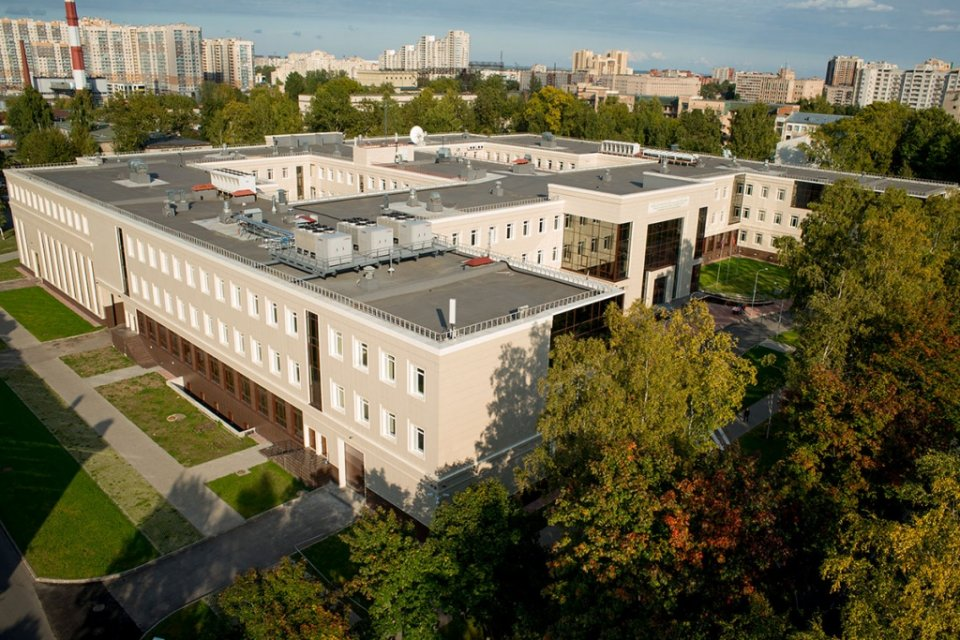
\includegraphics [scale=0.27] {my_folder/images/spbpu_new_bld_autumn}
%	\caption{Новый научно-исследовательский корпус СПбПУ \cite{spbpu-gallery}} 
%	\label{fig:spbpu-new-bld-autumn-ch2}  
%	\end{figure}
	


	
%\section{Название параграфа} \label{ch2:sec-abbr} %название по-русски
	
%Название параграфа оформляется с помощью команды \verb|\section{...}|, название главы --- \verb|\chapter{...}|. 
	

%\subsection{Название подпараграфа} \label{ch2:subsec-title-abbr} %название по-русски


%Название подпараграфа оформляется с помощью команды  \texttt{\textbackslash{}subsection\{...\}}.


%\subsubsection{Название подподпараграфа} \label{ch2:subsubsec-title-abbr} %название по-русски
	
%Использование подподпараграфов в основной части крайне не рекомендуется. В случае использования, необходимо вынести данный номер в содержание.	
%Название подпараграфа оформляется с помощью команды  \texttt{\textbackslash{}subsubsecti\-on\{...\}}.



%\input{my_folder/tex/enumeration} % правила использования перечислений	

	
%Оформление псевдокода необходимо осуществлять с помощью пакета \verb|algorithm2e| в окружении \verb|algorithm|. Данное окружение интерпретируется в шаблоне как рисунок. Пример оформления псевдокода алгоритма приведён на \firef{alg:AlgoFDSCALING}. 
	
	
%\input{my_folder/tex/pseudocode-agl-DTestsFDScaling} % пример оформления псевдокода алгоритма 	

	
%\section{Название параграфа} \label{ch2:sec-very-short-title} %название по-русски


	
%\input{my_folder/tex/eq-equation-multilined} % пример оформления одиночной формулы в несколько строк

%\input{my_folder/tex/fig-spbpu-sc-four-in-one} % пример подключения 4х иллюстраций в одном рисунке

%\input{my_folder/tex/fig-spbpu-whitehall-three-in-one} % пример подключения 3х иллюстрации в одном рисунке
%
%\input{my_folder/tex/fig-spbpu-main-bld-two-in-one} % пример подключения 2х иллюстраций в одном рисунке

%\input{my_folder/tex/tab-more-than-one-page} % пример подключения таблицы на несколько страциц




%% please, before using, read the author guide carefully

%\input{my_folder/tex/tab-toy-context-minipage} % пример подключения minipage

%\input{my_folder/tex/fig-spbpu-new-bld-autumn-minipage} % пример подключения minipage




%\input{my_folder/tex/rules-theorem-like-expressions} 

%По аналогии с нумерацией формул, рисунков и таблиц нумеруются и иные текстово-графические объекты, то есть включаем в нумерацию номер главы, например: теорема 3.1. для первой теоремы третьей главы монографии. Команды \LaTeX{} выставляют нумерацию и форматирование автоматически. Полный перечень команд для подготовки текстово-графических и иных объектов находится в подробных методических рекомендациях \cite{spbpu-bci-template-author-guide}. 


%\input{my_folder/tex/rules-list-of-environments} % список некоторых окружений


%\input{my_folder/tex/theorem-example} %пример оформления теоремы


%\input{my_folder/tex/definition-example} %пример оформления определения


%Вместо теоремо-подобных окружений для вставки небольших текстово-графических объектов иногда используются команды. Типичным примером такого подхода является команда \verb|\footnote{text}|\footnote{Внимание! Команда вставляется непосредственно после слова, куда вставляется сноска (без пробела). Лишние пробелы также не указываются внутри команды перед и после фигурных скобок.}, где в аргументе \verb|text| указывают текст \textit{подстрочной ссылки (сноски)}.В них \textit{нельзя добавлять веб-ссылки или цитировать литературу}. Для этих целей используется список литературы. Нумерация сносок сквозная по ВКР без точки на конце выставляется в шаблоне автоматически, однако в каждом приложении к ВКР нумерация, зависящая от номера приложения, выставляется префикс <<П>>, например <<П1.1>> --- первая сноска первого приложения. 




%\FloatBarrier % заставить рисунки и другие подвижные (float) элементы остановиться


%\section{Выводы} \label{ch2:conclusion}

%Текст заключения ко второй главе. Пример ссылок \cite{Article,Book,Booklet,Conference,Inbook,Incollection,Manual,Mastersthesis,Misc,Phdthesis,Proceedings,Techreport,Unpublished,badiou:briefings}, а также ссылок с указанием страниц, на котором отображены те или иные текстово-графические объекты  \cite[с.~96]{Naidenova2017} или в виде мультицитаты на несколько источников \cites[с.~96]{Naidenova2017}[с.~46]{Ganter1999}. Часть библиографических записей носит иллюстративный характер и не имеет отношения к реальной литературе. 

%Короткое имя каждого библиографического источника содержится в специальном файле \verb|my_biblio.bib|, расположенном в папке \verb|my_folder|. Там же находятся исходные данные, которые с помощью программы \texttt{Biber} и стилевого файла \texttt{Biblatex-GOST} \cite{ctan-biblatex-gost} приведены в списке использованных источников согласно ГОСТ 7.0.5-2008.
%Многообразные реальные примеры исходных библиографических данных можно посмотреть по ссылке \cite{ctan-biblatex-gost-examples}.

%Как правило, ВКР должна состоять из четырех глав. Оставшиеся главы можно создать по образцу первых двух и подключить с помощью команды \verb|\input| к исходному коду ВКР. Далее в приложении \ref{appendix-MikTeX-TexStudio} приведены краткие инструкции запуска исходного кода ВКР \cite{latex-miktex,latex-texstudio}.

%В приложении \ref{appendix-extra-examples} приведено подключение некоторых текстово-графических объектов. Они оформляются по приведенным ранее правилам. В качестве номера структурного элемента вместо номера главы используется <<П>> с номером главы. Текстово-графические объекты из приложений не учитываются в реферате.



%% Вспомогательные команды - Additional commands
%
%\newpage % принудительное начало с новой страницы, использовать только в конце раздела
%\clearpage % осуществляется пакетом <<placeins>> в пределах секций
%\newpage\leavevmode\thispagestyle{empty}\newpage % 100 % начало новой страницы